\subsection{\Mol}\label{sec:app_molpcba}

Accurate prediction of the biochemical properties of small molecules can  significantly accelerate drug discovery by reducing the need for expensive lab experiments \citep{shoichet2004virtual,hughes2011principles}.
However, the experimental data available for training such models is limited compared to the extremely diverse and combinatorially large universe of candidate molecules that we would want to make predictions on \citep{bohacek1996art,sterling2015,lyu2019ultra,mccloskey2020machine}.
This means that models need to generalize to out-of-distribution molecules that are structurally different from those seen in the training set.

We study this issue through the \Mol dataset, which is directly adopted from the Open Graph Benchmark~\citep{hu2020open} and originally curated by  MoleculeNet~\citep{wu2018moleculenet}.

\subsubsection{Setup}

\paragraph{Problem setting.}
We consider the domain generalization setting, where the domains are molecular scaffolds, and our goal is to learn models that generalize to structurally distinct molecules with scaffolds that are not in the training set (\reffig{dataset_molpcba}).
This is a multi-task classification problem: for each molecule, we predict the presence or absence of 128 kinds of biological activities, such as binding to a particular enzyme.
In addition, we cluster the molecules into different scaffold groups according to their two-dimensional structure, and annotate each molecule with the scaffold group that it belongs to.
Concretely, the input $x$ is a molecular graph, the label $y$ is a 128-dimensional binary vector where each component corresponds to a biochemical assay result, and the domain $d$ specifies the scaffold. Not all biological activities are measured for each molecule, so $y$ can have missing values.

\paragraph{Data.}
\Mol contains more than 400K small molecules with 128 kinds of prediction labels.
Each small molecule is represented as a graph, where the nodes are atoms and the edges are chemical bonds.
The molecules are pre-processed using \textsc{RDKit} \citep{landrum2006rdkit}.
Input node features are 9-dimensional, including atomic number, chirality, whether the atom is in the ring. Input edge features are 3-dimensional, including bond type and bond stereochemistry.

We split the dataset by scaffold structure. This \emph{scaffold split}~\citep{wu2018moleculenet} is also used in the Open Graph Benchmark~\citep{hu2020open}.
By attempting to separate structurally different molecules into different subsets, it provides a realistic estimate of model performance in prospective experimental settings.
We assign the largest scaffolds to the training set to make it easier for algorithms to leverage scaffold information, and the smallest scaffolds to the test set to ensure that it is maximally diverse in scaffold structure:
\begin{enumerate}
  \item \textbf{Training:} The largest 44,930 scaffolds, with an average of 7.8 molecules per scaffold.
  \item \textbf{Validation (OOD):} The next largest 31,361 scaffolds, with an average of 1.4 molecules per scaffold.
  \item \textbf{Test (OOD):} The smallest 43,793 scaffolds, which are all singletons.
\end{enumerate}

In \reffig{molpcba-task-analysis} (A), we plot the statistics of the scaffolds in terms of the number of molecules belonging to each scaffold. We see that the scaffold sizes are highly skewed, with the test set containing (by design) the scaffolds with the least molecules.
However, the differences in scaffold sizes do not significantly change the statistics of the molecules in each split.
In Figures \ref{fig:molpcba-task-analysis} (B) and (C), we see that the label statistics remain very similar across train/validation/test splits, suggesting that the main distribution shift comes from the difference in the input molecular graph structure.


\begin{figure*}[tbp]
  \centering
  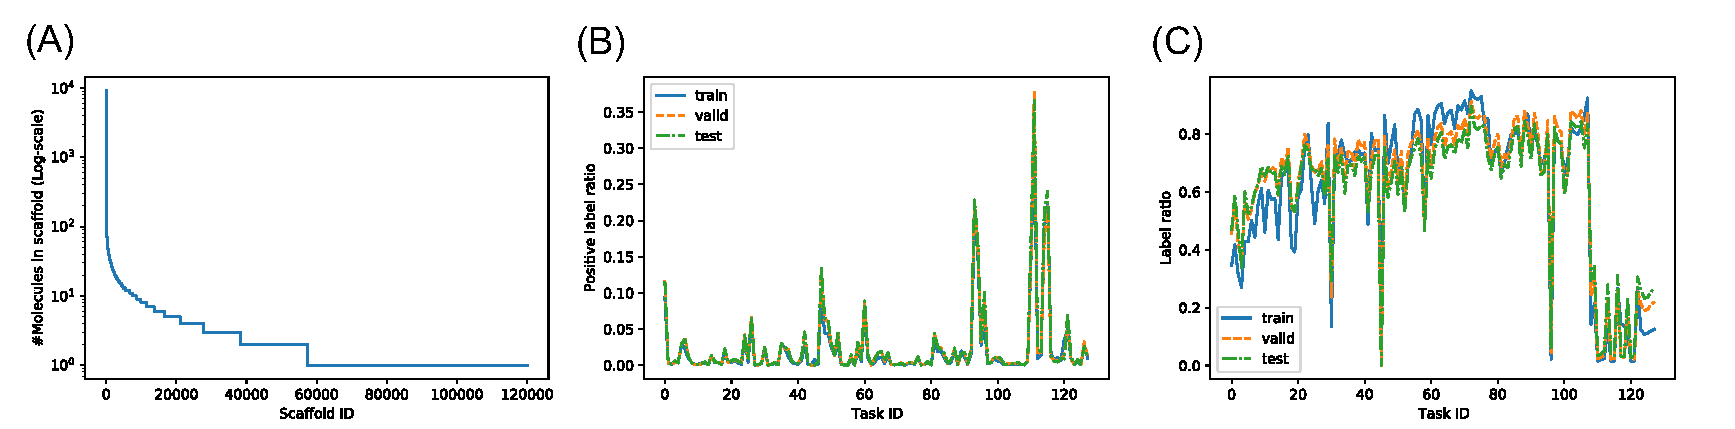
\includegraphics[width=\textwidth]{figures/molpcba_task_analysis.pdf}
  \caption{Analyses of scaffold groups in the \Mol dataset. (A) shows the distribution of the scaffold sizes, (B) and (C) show how the ratios of positive molecules and labeled molecules for the 128 tasks vary across the train/validation /test splits.}\label{fig:molpcba-task-analysis}
\end{figure*}


\paragraph{Evaluation.}
We evaluate models by their average Average Precision (AP) across tasks (i.e., we compute the average precision for each task separately, and then average those scores), following \citet{hu2020open}. This accounts for the extremely skewed class balance in \Mol (only 1.4\% of data is positive). Not all labels are available for each molecule; when calculating the AP for each task, we only consider the labeled molecules for the task.

\paragraph{Potential leverage.}
We provide the scaffold grouping of molecules for training algorithms to leverage. Finding generalizable representations of molecules across different scaffold groups is useful for models to make accurate extrapolation on unseen scaffold groups. In fact, very recent work~\citep{jin2020domain} has leveraged scaffold information of molecules to improve the extrapolation performance of molecular property predictors.

One notable characteristic of the scaffold group is that the size of each group is rather small; on the training split, each scaffold contains only 7.8 molecules on average. This also results in many scaffold groups: 44,930 groups in the training split. In \reffig{molpcba-task-analysis}, we show that these scaffold groups are well-behaved in the sense that the train/validation/test splits contain contain similar ratios of positive labels as well as missing labels.



\begin{table*}[t]
  \caption{Baseline results on \Mol. Parentheses show standard deviation across 3 replicates.}
  \label{tab:results_molpcba}
  \centering
  \begin{tabular}{lllcccc}
  \toprule
  Algorithm &  Validation AP (\%) & Test AP (\%) \\
  \midrule
  ERM &  \textbf{27.8} \std{0.1}  & \textbf{27.2} \std{0.3} \\
  CORAL &  18.4 \std{0.2} & 17.9 \std{0.5} \\
  IRM &  15.8 \std{0.2} & 15.6 \std{0.3} \\
  Group DRO &  23.1 \std{0.6} & 22.4 \std{0.6} \\
  \bottomrule
  \end{tabular}
\end{table*}

\begin{table*}[t]
  \caption{
  Random split comparison for ERM models on \Mol.
  In the official OOD setting, we train on molecules from some scaffolds and evaluate on molecules from different scaffolds, whereas in the random split setting, we randomly divide molecules into training and test sets without using scaffold information.
  Parentheses show standard deviation across 3 replicates.
  }
  \label{tab:drop_molpcba}
  \centering
  \begin{tabular}{lllcccc}
  \toprule
  Setting                              & Algorithm &  Test AP (\%) \\
  \midrule
  Official     (split by scaffolds)    & ERM & 27.2 \std{0.3} \\
  Random split (split i.i.d.)          & ERM & \textbf{34.4} \std{0.9} \\
  \bottomrule
  \end{tabular}
\end{table*}



\subsubsection{Baseline results}

\paragraph{Model.}
For all experiments, we use Graph Isomorphism Networks (GIN)~\citep{xu2018powerful} combined with virtual nodes~\citep{gilmer2017neural}, as this is currently the model with the highest performance in the Open Graph Benchmark~\citep{hu2020open}.
We follow the same hyperparameters as in the Open Graph Benchmark: 5 GNN layers with a dimensionality of 300;
the Adam optimizer \citep{kingma2014adam} with a learning rate of 0.001;
and training for 100 epochs with early stopping.
For each of the baseline algorithms (ERM, CORAL, IRM, and Group DRO),
we separately tune the dropout rate from $\{0, 0.5\}$;
in addition, for CORAL and IRM, we tune the penalty weight as in \refapp{experiments}.

\paragraph{ERM results and performance drops.}
We first compare the generalization performance of ERM on the official scaffold split against the conventional random split, in which the entire molecules are randomly split into train/validation/test sets with the same split ratio as the scaffold split (i.e., 80/10/10).
Results are in \reftab{drop_molpcba}. The test performance of ERM drops by 7.2 points AP when the scaffold split is used, suggesting that the scaffold split is indeed harder than the random split.

To maintain consistency with the Open Graph Benchmark, and because the number of examples (molecules) per domain (scaffold) is relatively small compared to other datasets, we opted not to split off a portion of the training set into Validation (ID) and Test (ID) sets.
We therefore do not run a train-to-train comparison for \Mol.
Moreover, as the official scaffold split assigns the largest scaffolds to the training set and the smallest scaffolds to the test set, the test scaffolds all only have one molecule per scaffold, which precludes running test-to-test and mixed-to-test comparisons.

A potential issue with the random split ID comparison is that it does not measure performance on the same test distribution as the official split, and therefore might be confounded by differences in intrinsic difficulty. However, we believe that the random split setting provides a reasonable measure of ID performance for \Mol, as \reffig{molpcba-task-analysis} shows that the distribution of scaffolds assigned to the training versus test sets are similar. As the random split contains many singleton scaffolds in its test set that do not have corresponding molecules in the training set, we believe that it is likely to be an underestimate of the ID-OOD gap in \Mol.

\paragraph{Additional baseline methods.}
\reftab{results_molpcba} also shows that ERM performs better than CORAL, IRM, and Group DRO, all of which use scaffolds as the domains. For CORAL and IRM, we find that smaller penalties give better generalization performance, as larger penalty terms make the training insufficient.
We use the $0.1$ penalty for CORAL and $\lambda=1$ for IRM.

The primary issue with these existing methods is that they make the model significantly underfit the training data even when dropout is turned off.
For instance, the training AP of CORAL and IRM is 20.0\% and 15.9\%, respectively, which are both lower than the 36.1\% that ERM obtains even with 0.5 dropout.
Also, these methods are primarily designed for the case when each group contains a decent number of examples, which is not the case for the \Mol dataset.

\subsubsection{Broader context}
Because of the very nature of discovering \emph{new} molecules, out-of-distribution prediction is prevalent in nearly all applications of machine learning to chemistry domains. Beyond drug discovery, a variety of tasks and their associated datasets have been proposed for molecules of different sizes.

For small organic molecules, the scaffold split has been widely adopted to stress-test models' capability for out-of-distribution generalization. While \Mol primarily focuses on predicting biophysical activity (e.g., protein binding), other datasets in  MoleculeNet \citep{wu2018moleculenet} include prediction of quantum mechanical properties (e.g., HOMO/LUMO), physical chemistry properties (e.g., water solubility), and physiological properties (e.g., toxicity prediction \citep{attene2013tox21}).

Besides small molecules, it is also of interest to apply machine learning over larger molecules such as catalysts and proteins.
In the domain of catalysis, using machine learning to approximate expensive quantum chemistry simulation has gotten attention. The OC20 dataset has been recently introduced, containing 200+ million samples from quantum chemistry simulations relevant to the discovery of new catalysts for renewable energy storage and other energy applications~\citep{becke2014perspective,chanussot2020open,zitnick2020introduction}. The OC20 dataset explicitly provides test sets with qualitatively different materials.
In the domain of proteins, the recent trend is to use machine learning to predict 3D structure of proteins given their amino acid sequence information. This is known as the protein folding problem, and has sometimes been referred to as the Holy Grail of structural biology~\citep{dill2012protein}.
CASP is a bi-annual competition to benchmark the progress of protein folding~\citep{moult1995large}, and it evaluates predictions made on proteins whose 3D structures are identified very recently, presenting a natural temporal distribution shift.
Recently, the AlphaFold2 deep learning model obtained breakthrough performance on the CASP challenge~\citep{jumper2020alphafold}, demonstrating exciting avenues of machine learning for structural biology.


\subsubsection{Additional details}\label{sec:app_molpcba_details}
\textbf{Data processing.}
The \Mol dataset contains 437,929 molecules annotated with 128 kinds of labels, each representing a bioassay curated in the PubChem database~\citep{kim2016pubchem}. More details are provided in the MoleculeNet~\citep{wu2018moleculenet} and the Open Graph Benchmark~\citep{hu2020open}, from which the dataset is adopted.
